\begin{section}{Resultados}
	\begin{subsection}{Ajuste de parámetros}
		El algoritmo de $Newton$ utilizado para buscar los ceros de un polinomio hace uso de dos parámetros, los cuales tuvimos que ajustar de manera de conseguir los mejores resultados posibles, mejores en el sentido de relación calidad de la solución y eficiencia en terminos de tiempo del algoritmo.

		La siguientes pruebas se realizaron para ajustar el parámetro ($tolerancia$) del programa que sirve para buscar los $ceros$ de un polinomio y la máxima cantidad de iteraciones permitidas. El primer parámetro se utiliza para decidir si un valor es una raíz (más específicamente nos dice si estamos cerca del cero). La $tolerancia$ es definida como la distancia entre un par de puntos, que en nuestro caso corresponde a las posibles raíces
		
		Se muestra el siguiente gráfico para esclarecer el uso de este parámetro.
		
		\begin{figure}[H]
		  \centering
			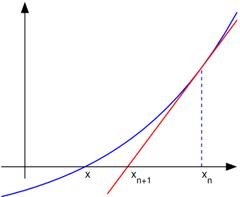
\includegraphics[width=5cm]{graficos/newton.jpg}
		  \caption{Método de Newton}
		  \label{fig:newton}
		\end{figure}
		
		En el gráfico anteriormente expuesto esta $tolerancia$ se define como el valor absoluto entre la diferencia entre $x_{n+1}$ y $x_n$. 
		Si el algortimo de $Newton$ termina porque consigue la $tolerancia$ pedida (no se le terminan las iteraciones permitidas) devuelve $x_{n+1}$ y la distancia entre $x_{n+1}$ y $x_n$ es menor a la $tolerancia$ ($x_{n+1} - x_n < tolerancia$).
				
		Como ya mencionamos, uno de los parámetros es para determinar la máxima cantidad de iteraciones que le permitimos al algoritmo buscar. 
		Para ajustar este parámetro elegimos de manera aleatorea $siete$ instancias (polinomios) y realizamos un gráfico de cantidad de iteraciones en función del error al cero teórico.

		\begin{figure}[H]
		  \centering
			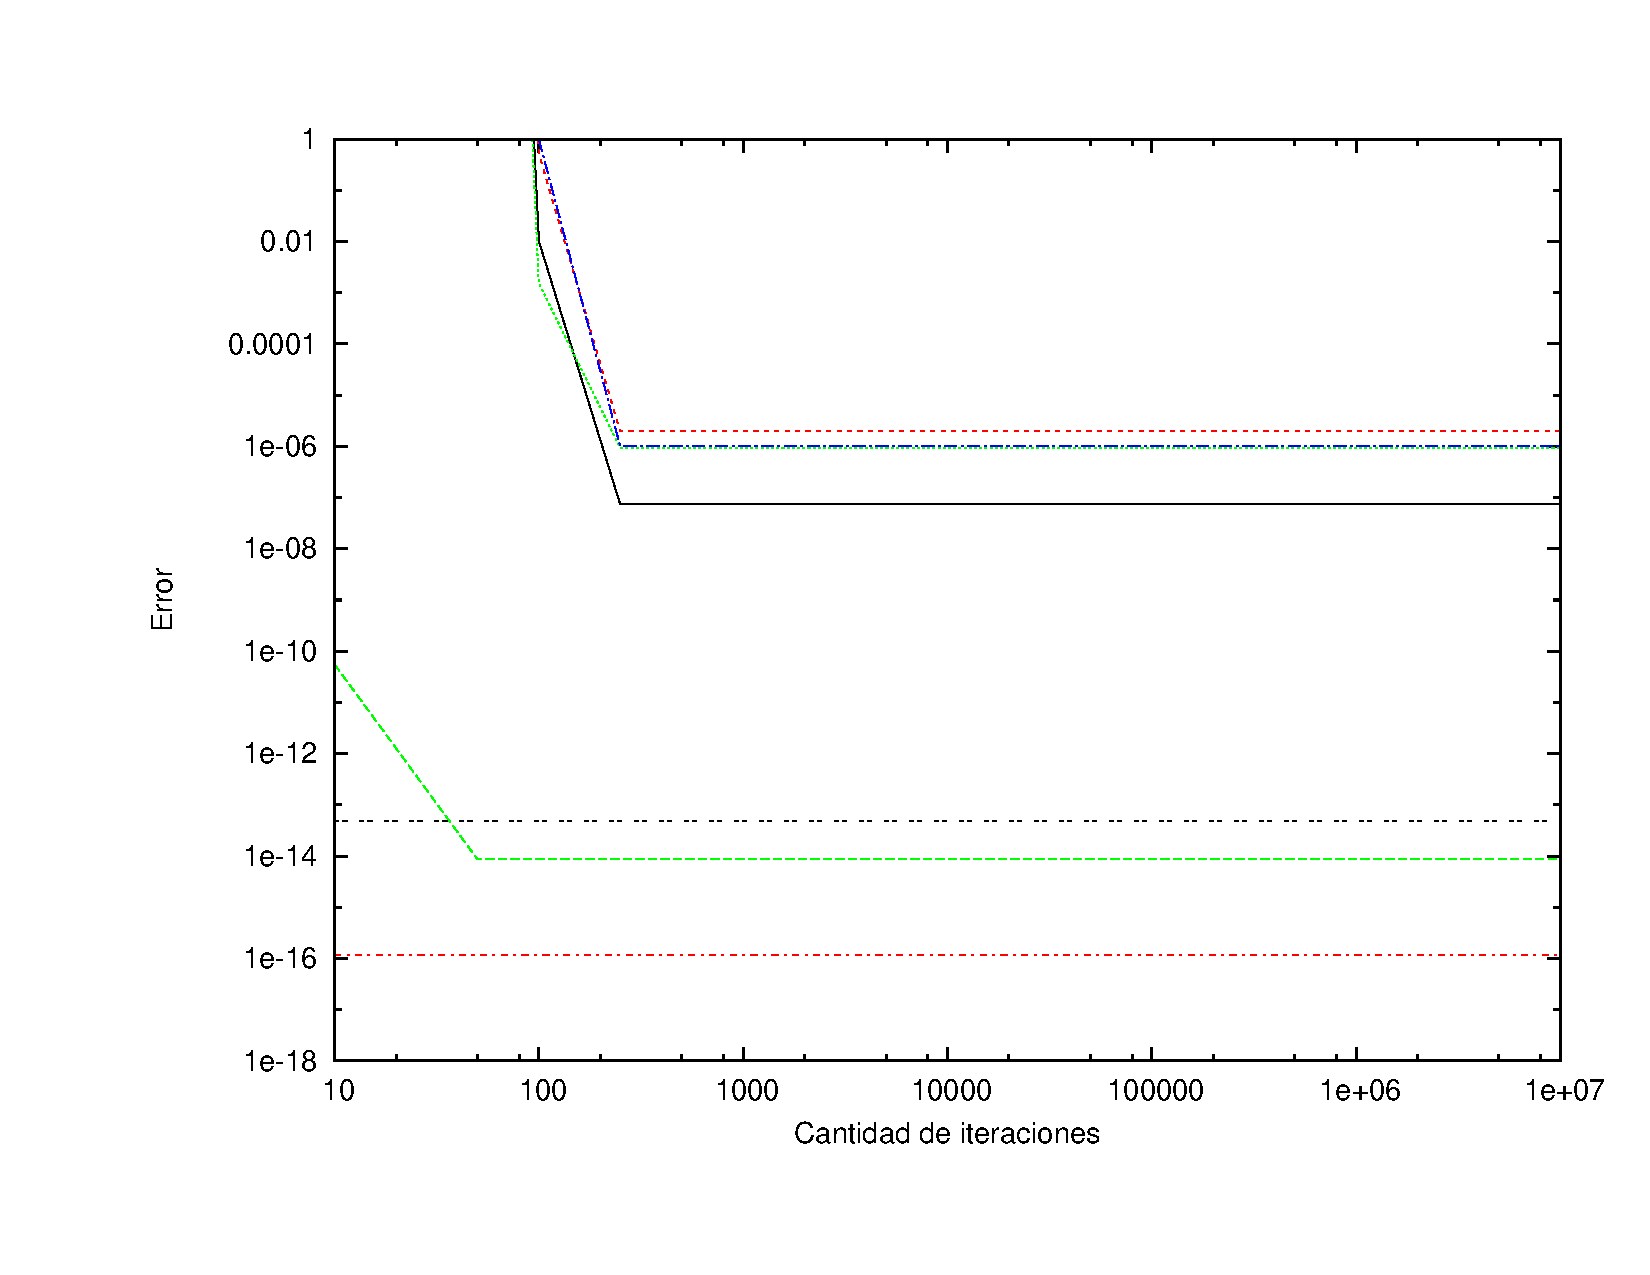
\includegraphics[width=14cm]{graficos/iter_graf.pdf}
		  \caption{Cantidad de iteraciones en función del error al cero teórico}
		  \label{fig:iter}
		\end{figure}

		Esperamos con este gráfico poder ver la cantidad de iteraciones promedio necesarias para que la solución puede considerarse correcta. Además esperamos poder dilucidar alguna relación entre la cantidad de iteraciones adecuadas y el valor de $toleracia$ óptimo al cero teórico.
		
		A continuación presentamos un nuevo gráfico utilizando ahora como coordenada $x$ el costo en cantidad de operaciones del algoritmo y como $y$ el error cometido, es decir la distancia a la raíz real. Se utilizaron para este $test$ treinta y cinco (35) instancias aleatoreas, para distintos valores de $tolerancia$: $1e^-1$, $1e^-3$, $1e^-5$, $1e^-9$, $1e^-13$, $1e^-17$ y $1e^-24$ (se utilizó un generador de polinomios creado por nosotros, eligiendo de manera 'random' cada coeficiente).
		
		El gráfico se presenta bajo escala logarítmica en $y$\\

		\begin{figure}[H]
		  \centering
			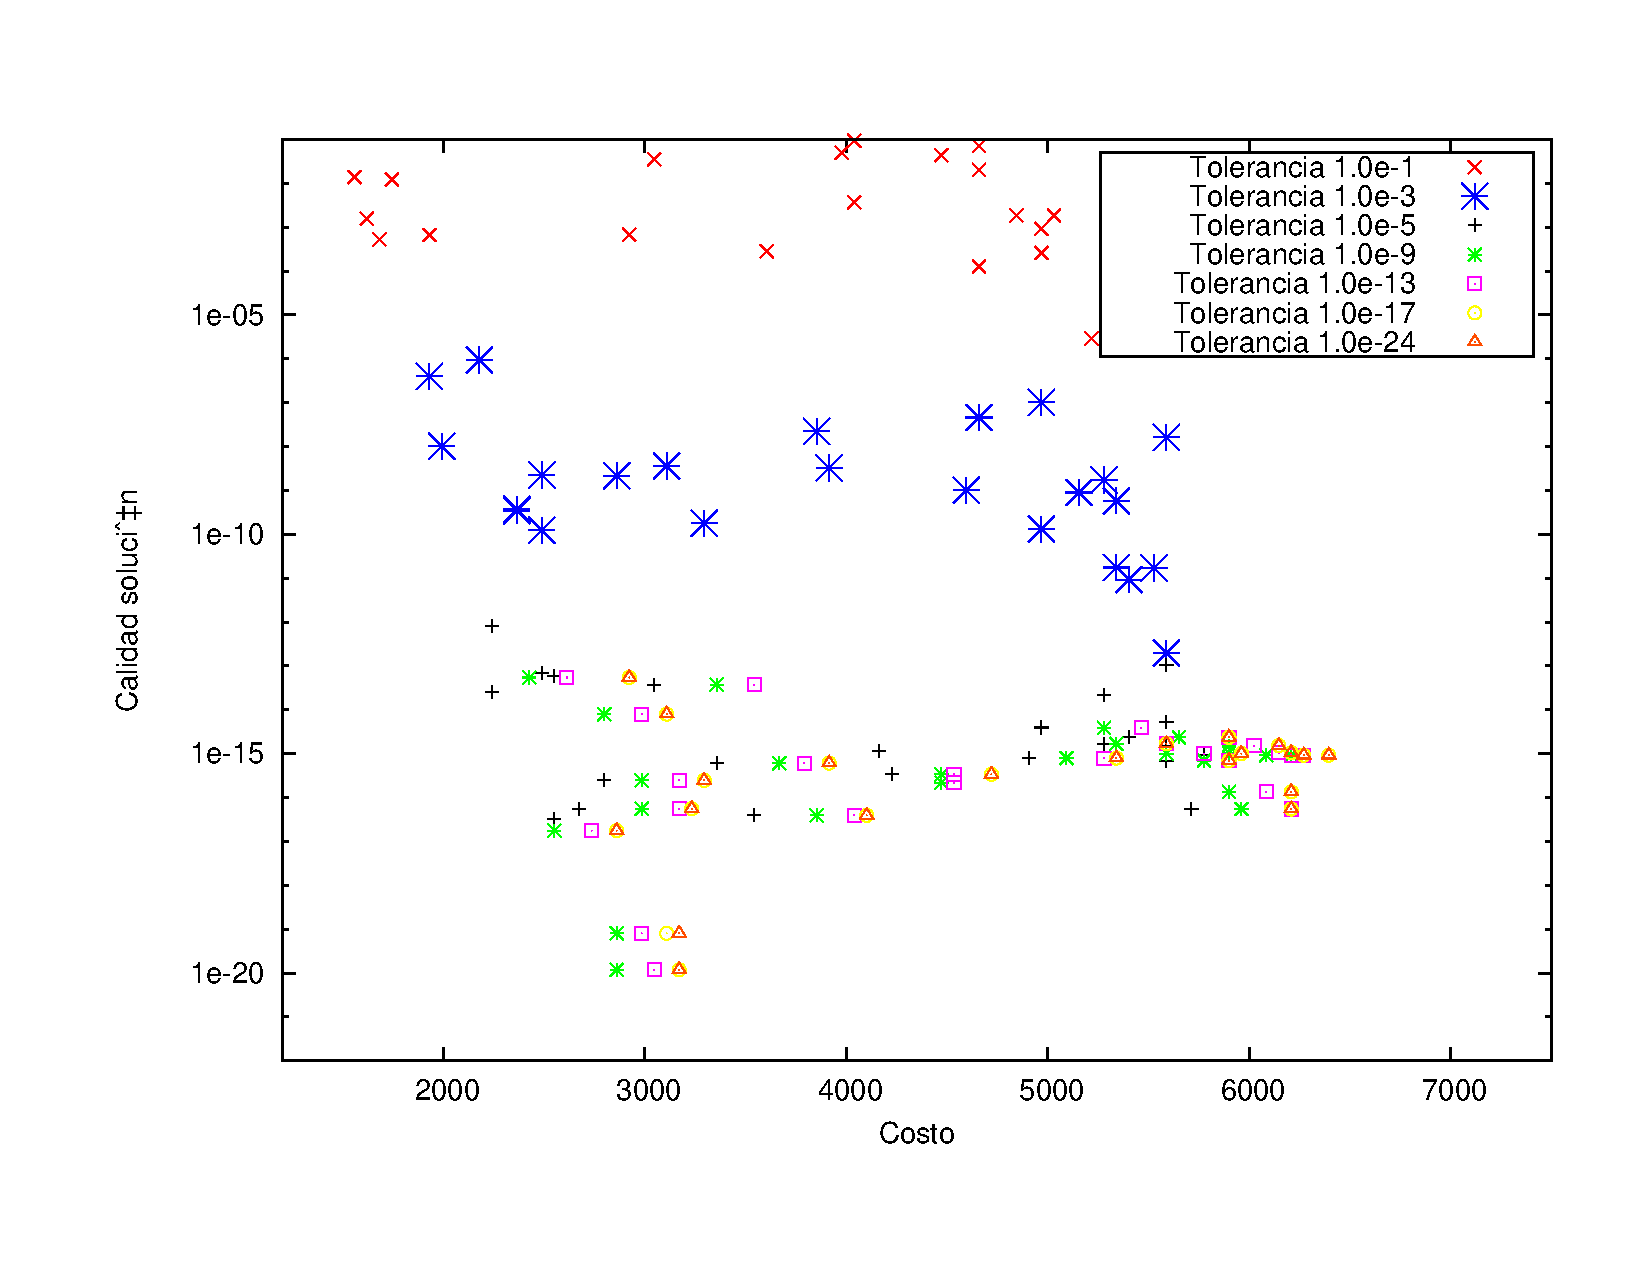
\includegraphics[width=14cm]{graficos/tol_graf.pdf}
		  \caption{Costo del algoritmo de Newton en función de la calidad de la solución variando el parámetro tolerancia}
		  \label{fig:5p_r}
		\end{figure}
		
		\VSP
		
		Esperamos ver que cuanto menor es la $tolerancia$ mejor es la aproximación al cero teórico. Recordar que el algoritmo que busca los ceros de un polinomio tiene dos criterios de parada (la tolerancia y la cantidad de iteraciones permitidas), creemos que la aproximación va a mejorar al disminuir la tolerancia ya que si termina por el primer motivo el valor conseguido va a ser igual o más refinado (más cercano a 0) y si lo hace por el segundo va a mejorar la aproximación durante más iteraciones. A pesar de esto, debemos buscar un equilibrio entre la calidad de la solución y el costo de la misma.\\
		
	\end{subsection}

	\begin{subsection}{Análisis de curvas}
		Para poder analizar si existen diferencias en el uso de distintas parametrizaciones se creó un generador de puntos de control a partir de un par de polinomios (uno para la coordenada $x$ y otra para $y$ que fueron elegidos de manera arbitraria) los cuales forman la curva. Los puntos de control pueden ser elegidos de forma aleatoria o uniforme. Graficamos entonces la curva con los puntos de control seleccionados de alguna de las dos formas anteriormente mencionadas, y las curvas utilizando las distintas de parametrizaciones (uniforme, por longitud de cuerda y centrípeta).
		
		Los siguientes gráficos utilizan un conjunto de cinco puntos de control aleatorios dada la misma curva.
				
		\begin{figure}[H]
		  \centering
			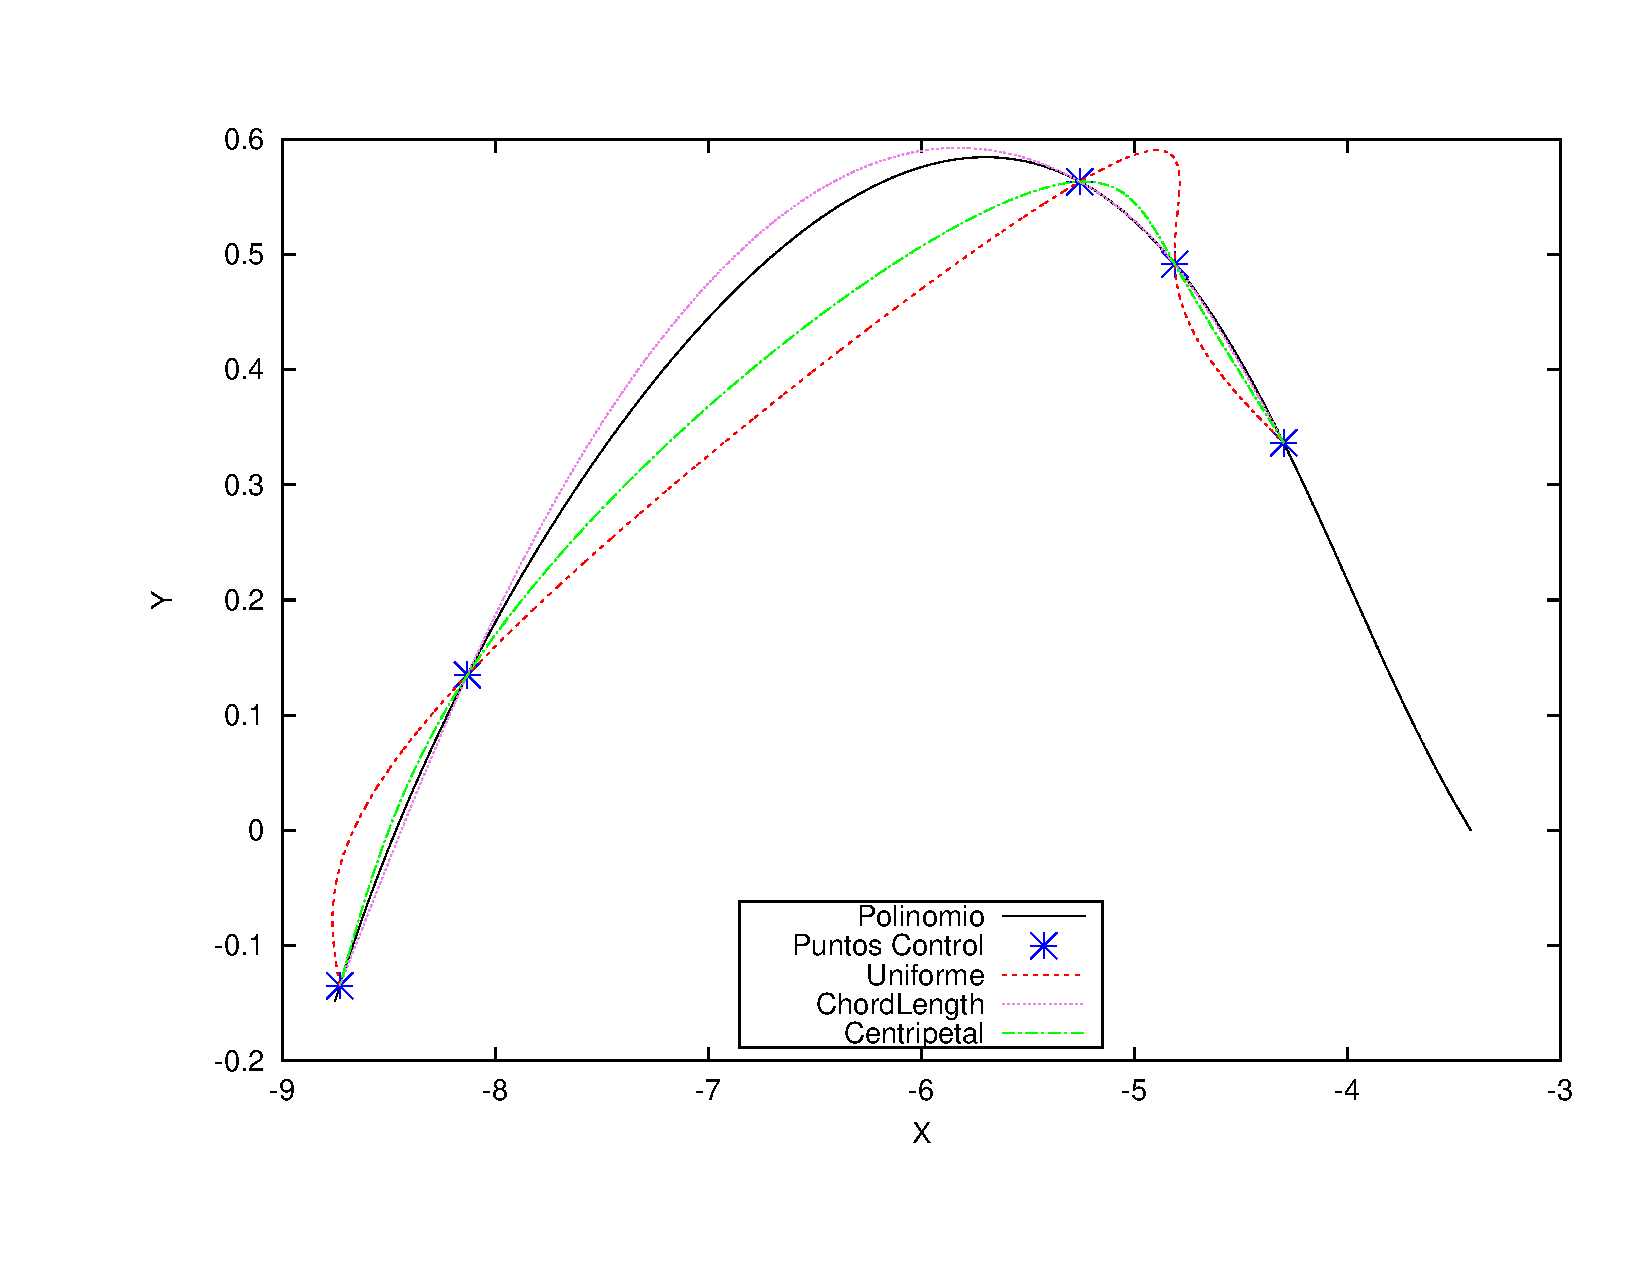
\includegraphics[width=14cm]{graficos/5p.pdf}
		  \caption{Aproximación por las distintas parametrizaciones utilizando cinco puntos de control aleatoreos}
		  \label{fig:5p}
		\end{figure}
		
		\VSP
		
		\begin{figure}[H]
		  \centering
			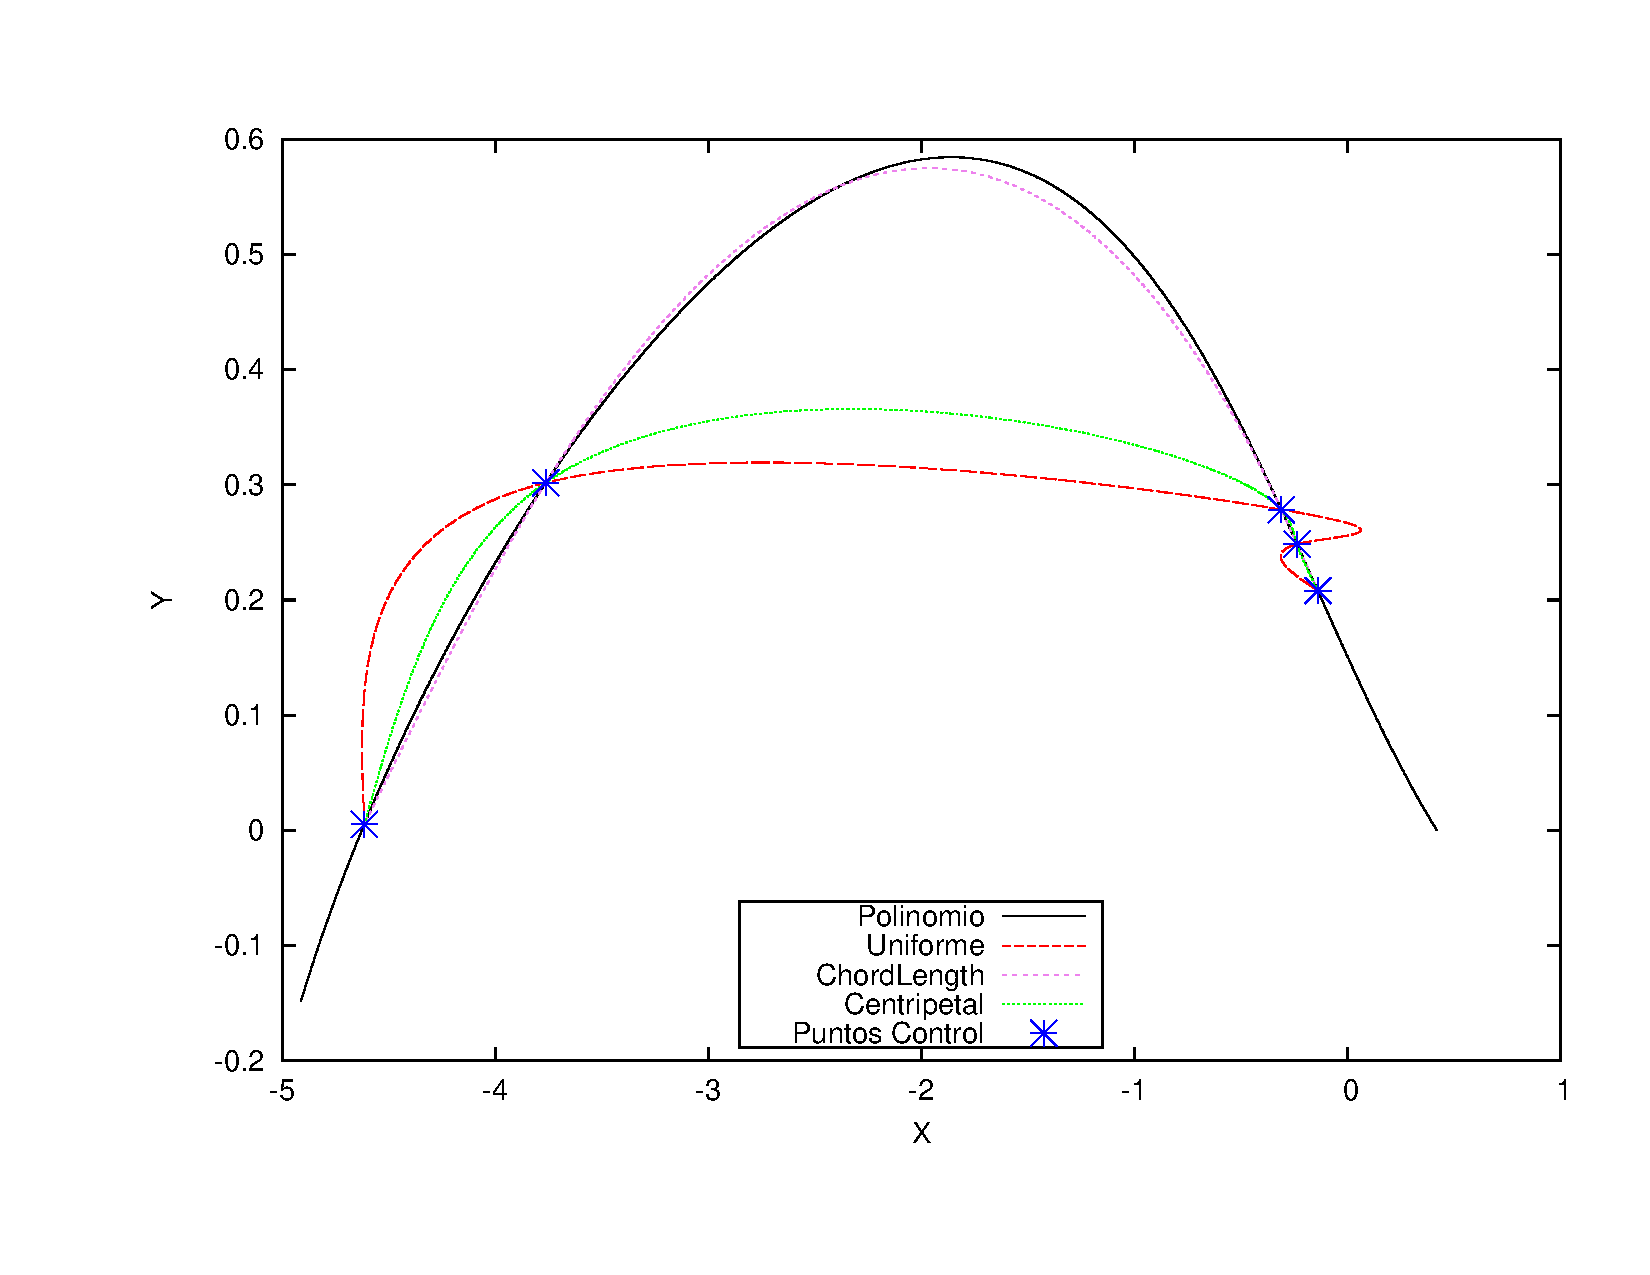
\includegraphics[width=14cm]{graficos/5p_r.pdf}
		  \caption{Aproximación por las distintas parametrizaciones utilizando cinco puntos de control aleatoreos}
		  \label{fig:5p_r}
		\end{figure}
		
		\VSP
		
		A continuación, se utiliza el mismo polinomio que el gráfico anterior pero tomando los puntos de control uniformemente.
		
		\begin{figure}[H]
		  \centering
			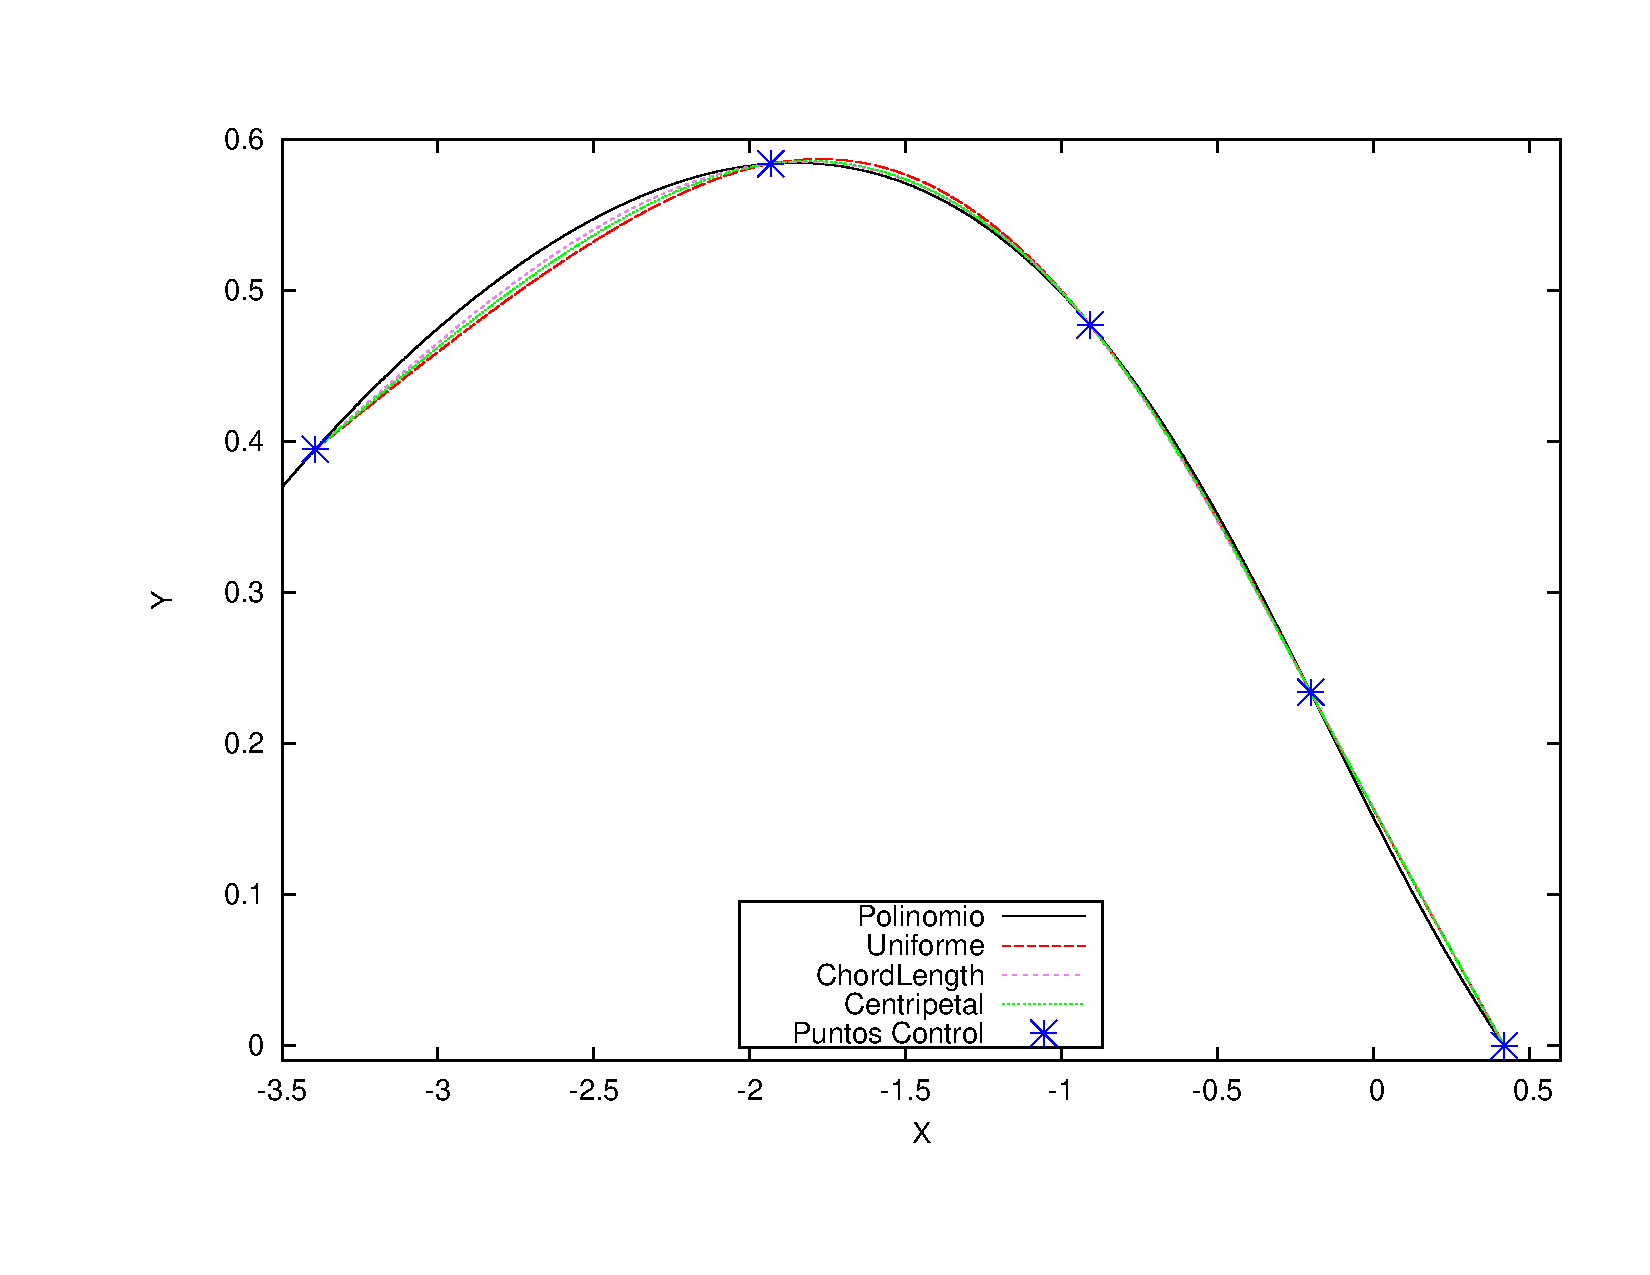
\includegraphics[width=14cm]{graficos/5p_u.pdf}
		  \caption{Aproximación por las distintas parametrizaciones utilizando cinco puntos distribuidos uniformemente}
		  \label{fig:5p_u}
		\end{figure}
		
		\VSP

		Los siguientes gráficos detallan cómo cambia la aproximación a una curva dada una parametrización a medida que se le provee más puntos de control. 
		Los puntos fueron tomados aleatoreamente y se utilizó la misma curva para las tres parametrizaciones para una comparación y análisis más claro.
			
		El primero de los gráficos muestra la variación en la aproximación para la parametrización uniforme.
			
		\begin{figure}[H]
		  \centering
			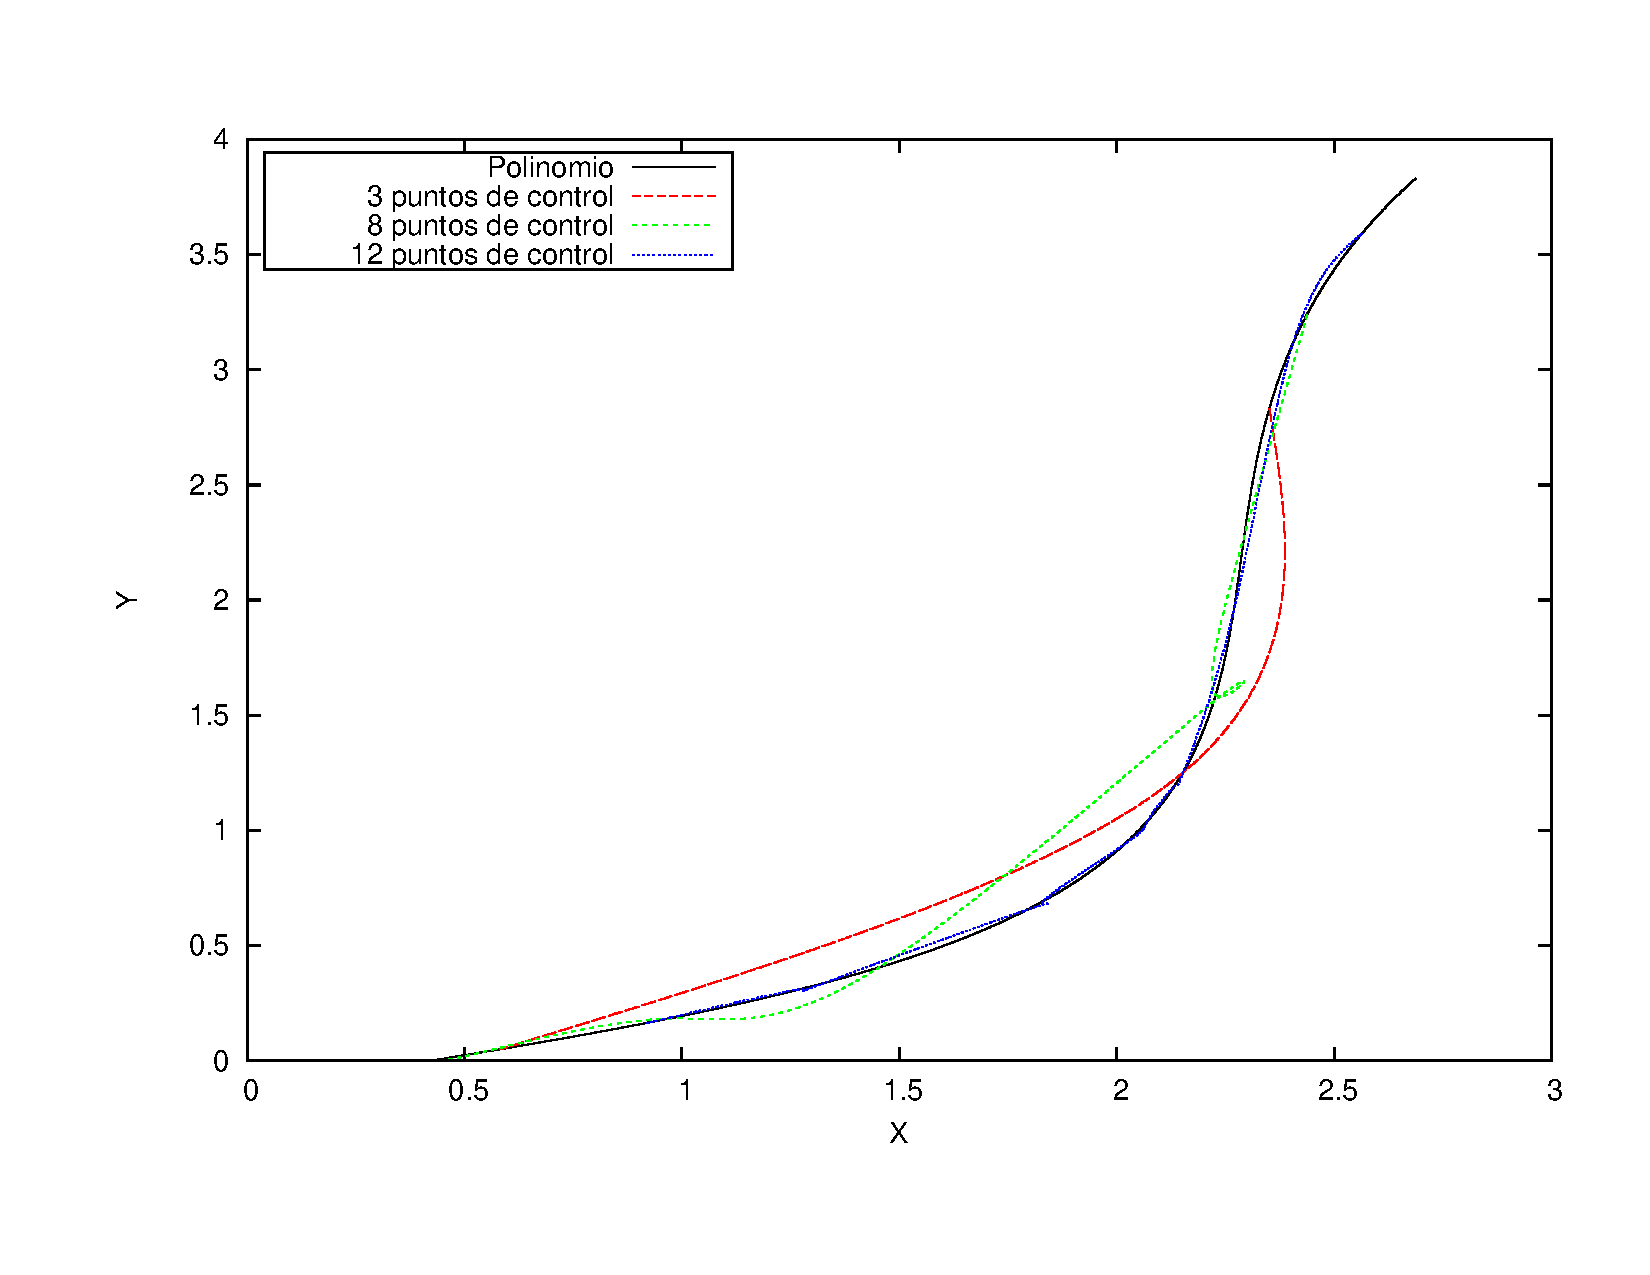
\includegraphics[width=14cm]{graficos/uniform_grafiquinSame.pdf}
		  \caption{Aproximación utilizando parametrización uniforme}
		  \label{fig:uniform}
		\end{figure}
		
		\VSP
		
		El siguiente gráficos muestra la variación en la aproximación para la parametrización centripeta.
		
		\begin{figure}[H]
		  \centering
			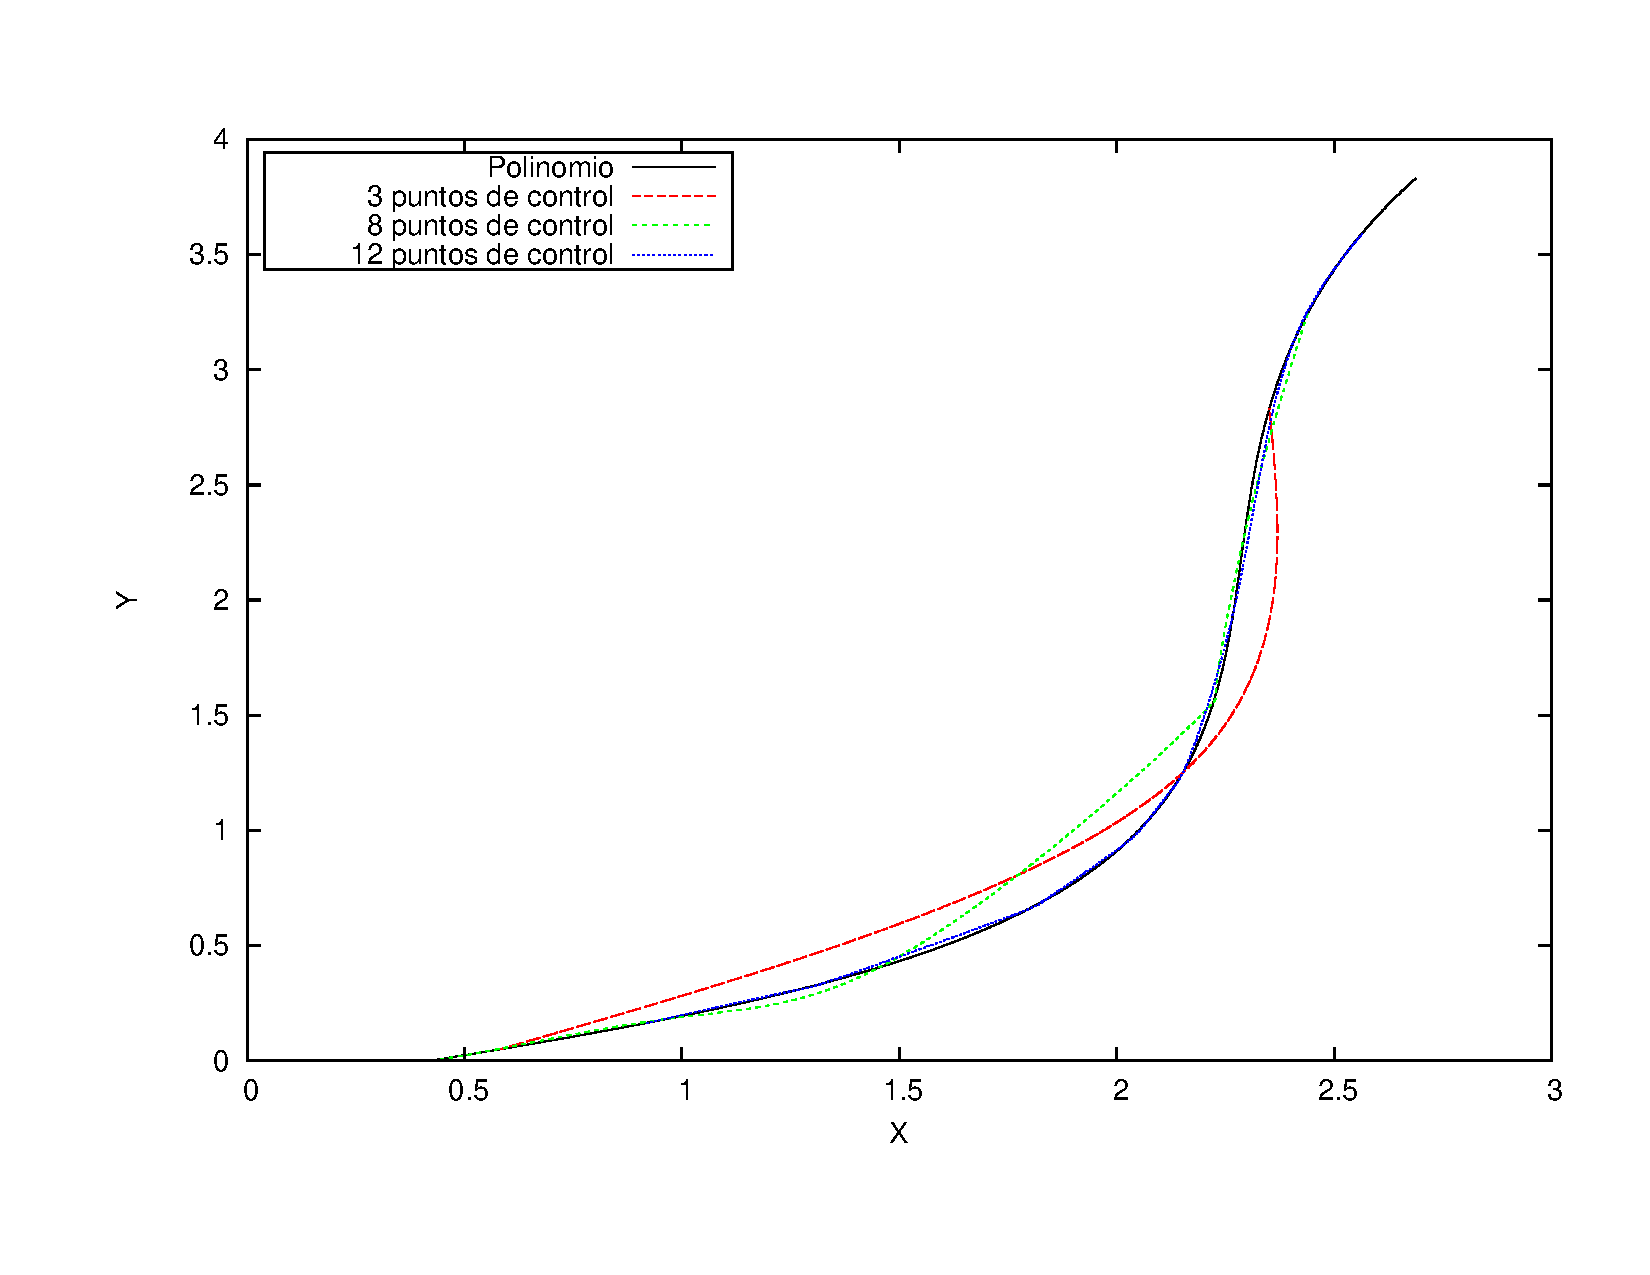
\includegraphics[width=14cm]{graficos/centripetal_grafiquinSame.pdf}
		  \caption{Aproximación utilizando parametrización centrípeta}
		  \label{fig:centripetal}
		\end{figure}
		
		\VSP

		Por último, se muestra la variación utilizando parametrización por longitud de cuerda.

		\begin{figure}[H]
		  \centering
			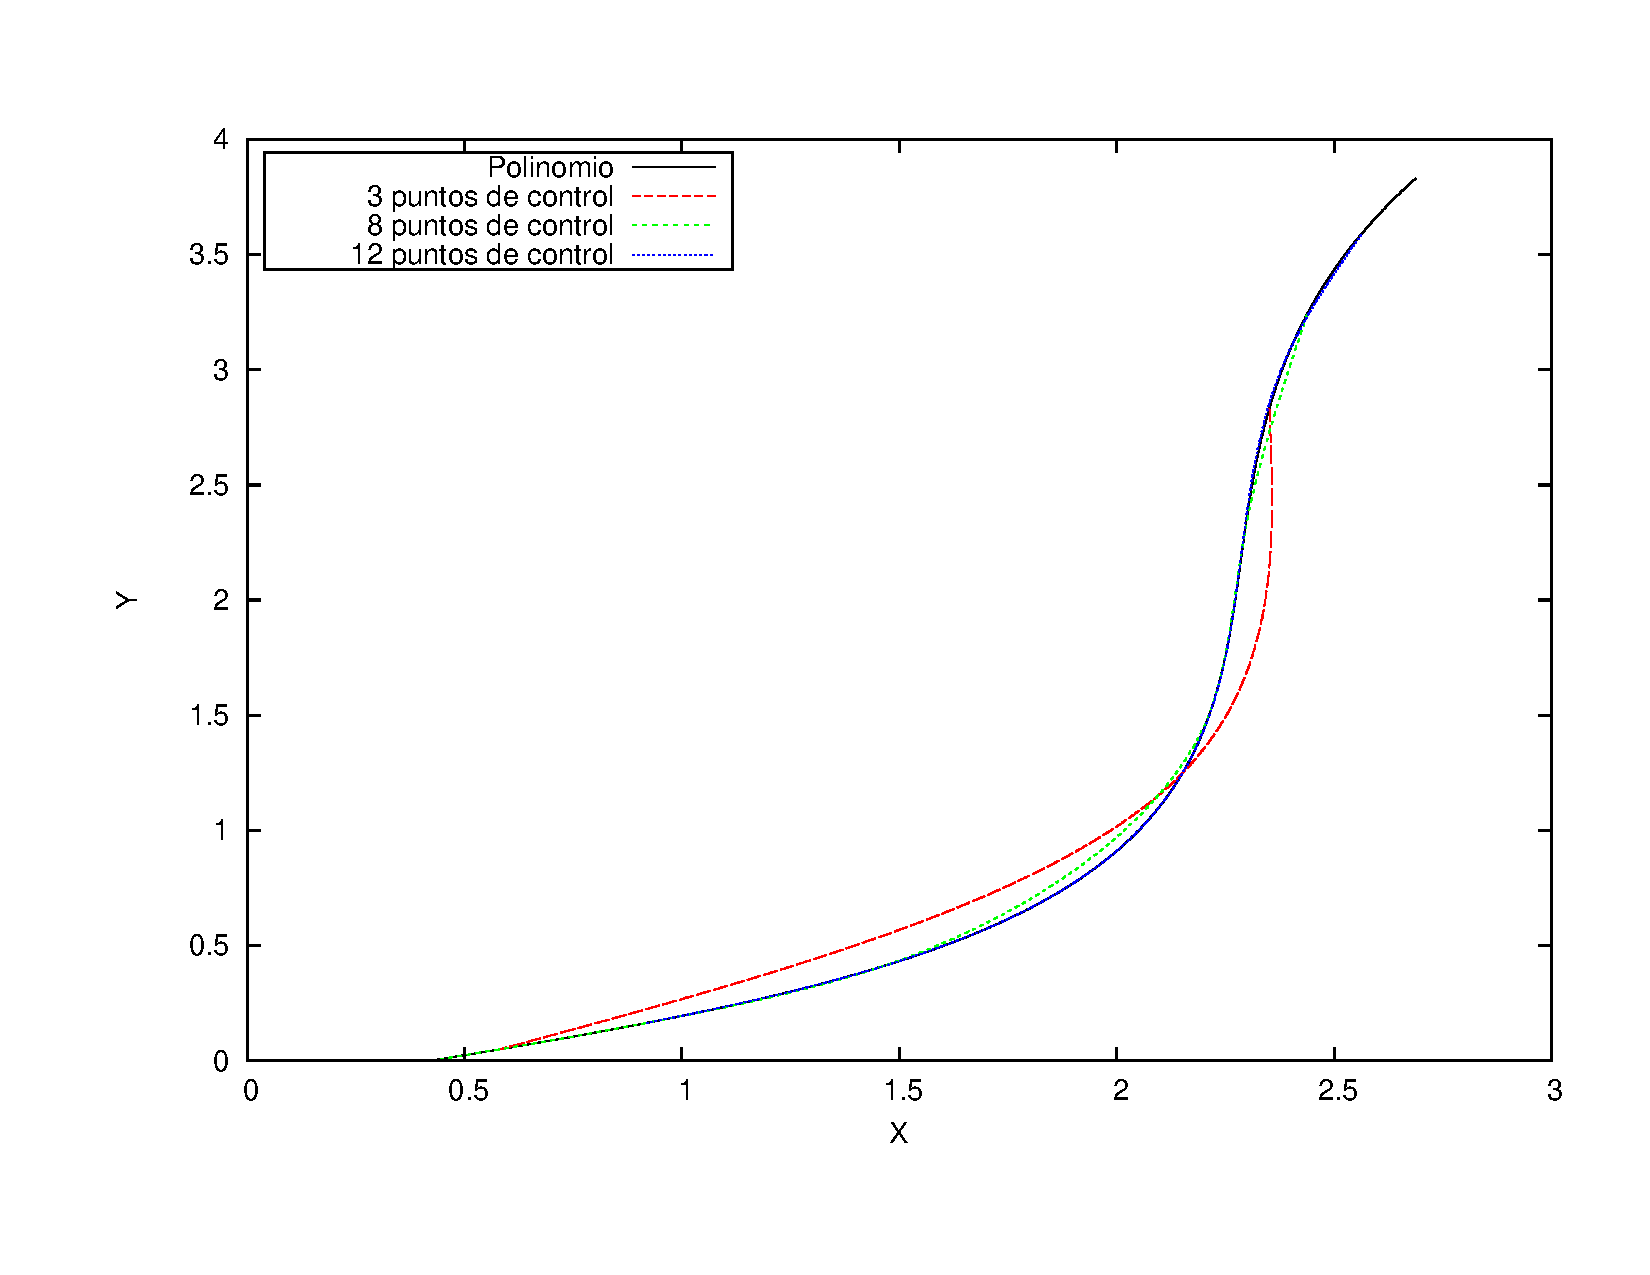
\includegraphics[width=14cm]{graficos/chordLength_grafiquinSame.pdf}
		  \caption{Aproximación utilizando parametrización por longitud de cuerda}
		  \label{fig:chordLength}
		\end{figure}
		
		\VSP
	\end{subsection}
\end{section}
